\PassOptionsToPackage{dvipsnames, table}{xcolor}
\documentclass[notitlepage, twocolumn, 12pt]{article}
\usepackage{mypackagesv2}
\usepackage{float}
\usepackage[tmargin=1in,bmargin=1in,lmargin=1in,rmargin=1in]{geometry}
\usepackage[dvipsnames]{xcolor}

\setlength{\belowcaptionskip}{-10pt}
\tolerance=1
\emergencystretch=\maxdimen
\hyphenpenalty=10000
\hbadness=10000


\title{Testing a Model to Predict the Motion of a Pendulum} % bad title fix
\author{Pranav Upreti | PHY 180 Lab 2 \small{\textcolor{Plum}{Purple is lab 2}, Black is lab 1, \textcolor{WildStrawberry}{Red is edits to lab 1}}}

\begin{document}
    \maketitle
    \begin{abstract}
        % ask about abstract
        % ask about tense
    A pendulum was constructed from household materials to test a damped harmonic oscillator model proposed by Brian Wilson \cite{Wilson}. The pendulum's Q factor was measured to be 270 $\pm$ 20 from release angles between $1.40 \pm 0.01$ rad to $-1.40 \pm 0.01$ rad.  With the same setup, the length of the pendulum string was varied and the pendulum's period was measured. The pendulum length and period are linearly proportional by the equation $T = (2.15 \pm 0.05)L^{0.44 \pm 0.06}$ which partially agrees with Wilson's prediction that $T = 2L^{0.5}$. The Q factor increased linearly with pendulum length by the equation $Q = (2.2 \pm 0.3)L + 80 \pm 10$. 
    
    These experimental results indicate that Wilson's model is most accurate for small release angles, but quadratic damping forces like drag should be considered to improve this model. % to improve the results, can be improved with equipment out of the scope of this project. % should probably define Q,T,L???

    \end{abstract}
    \section*{Introduction}
    \color{Plum}
    This lab was split into three experiments. Part (i) tested the symmetry of the pendulum setup by comparing periods of positive and negative angles with equal magnitude. A period-angle graph was plotted and an order 2 power series was fit:  $T_O(1+B\theta_0+C\theta_0^2)$.
    
    Part (ii) used the same setup as part (i) to determine its $Q$ factor. The $Q$ factor is a constant which describes how quickly the pendulum's amplitude of oscillation decays(see background), and can be calculated two ways. First, by using decay constant found by applying an exponential curve fit to an amplitude-time graph, and the relation $Q=\nicefrac{\pi\tau}{T}$, where $T$ is the period and $\tau$ is a decay constant found from the curve fit. It can also be counted by measuring the number of oscillations until it decays to $e^{-\pi}$ of its initial amplitude (see background) \cite{Wilson}.
    
    Part (iii)a tested for a relation between the pendulum's length and period. A plot of pendulum length against period was fit to $T = kL^n$, where $L$ is the length of the string and $k,n$ are constants. Wilson predicts that $k \approx 2$ and $ n \approx 0.5$.

    Part (iii)b uses the data from part (iii)a to plot $Q$ factor against pendulum length. It was fit against first and second order power series, exponential, and logarithmic functions.  

    \subsection*{Background}
    \color{WildStrawberry}
    Pendulums and other oscillating systems decay in amplitude over time. Wilson suggests this is due to a damping force linearly proportional the velocity of the pendulum mass, call it $-b\diff{x}{t}$ where $b$ is a constant, $x$ is a particle's displacement from equilibrium, and $t$ is time \cite{OpenStax}. We use this to begin deriving Wilson's model:
    \begin{align*}
        m \diff[2]{x}{t} &= - b \diff{x}{t} - kx \\
        \intertext{where $b$ is some constant, and $k$ is the spring constant of the rope. Rearrange to obtain,}
        0 &= m \diff[2]{x}{t} + b \diff{x}{t} + kx   \\
    \intertext{this is a linear differential equation \cite{OpenStax} whose solution is} 
        x(t) &= A_0e^{\nicefrac{-bt}{2m}}\cos(\omega t + \phi)
    \end{align*} 
    Wilson's model is equivalent and predicts angle with time instead of position. As well, it introduces a constant $\nicefrac{1}{\tau} = \nicefrac{b}{2m}$ and uses $\omega = \nicefrac{2 \pi}{T}$ to get the equation:
    \begin{equation}\label{eq:1}
        \theta(t) = \theta_0 e^{-\nicefrac{t}{\tau}}\cos(\nicefrac{2\pi}{T} + \phi)
    \end{equation}
    The exponential decay in amplitude this model predicts is quantified by a constant called the $Q$ factor;  $Q \vcentcolon= \nicefrac{\pi \tau}{T}$. $Q$ can be calculated by finding $\tau$ from experimental data and substituting it into $Q = \nicefrac{\pi \tau}{T}$, or by measuring the number of oscillations until the amplitude of oscillation is $\theta_0e^{-\pi}$. Both methods were used to calculate $Q$. 
    
    
    \section*{Methodology} \label{method}

    \textcolor{Plum}{A pendulum, shown in \cref{fig:setup}, was constructed to test for (i) symmetry in the pendulum setup, (ii) the $Q$ factor of the pendulum and (iii) a relationship between the length of the pendulum, the $Q$ factor, and the pendulum period.}
    \begin{figure}[H]
        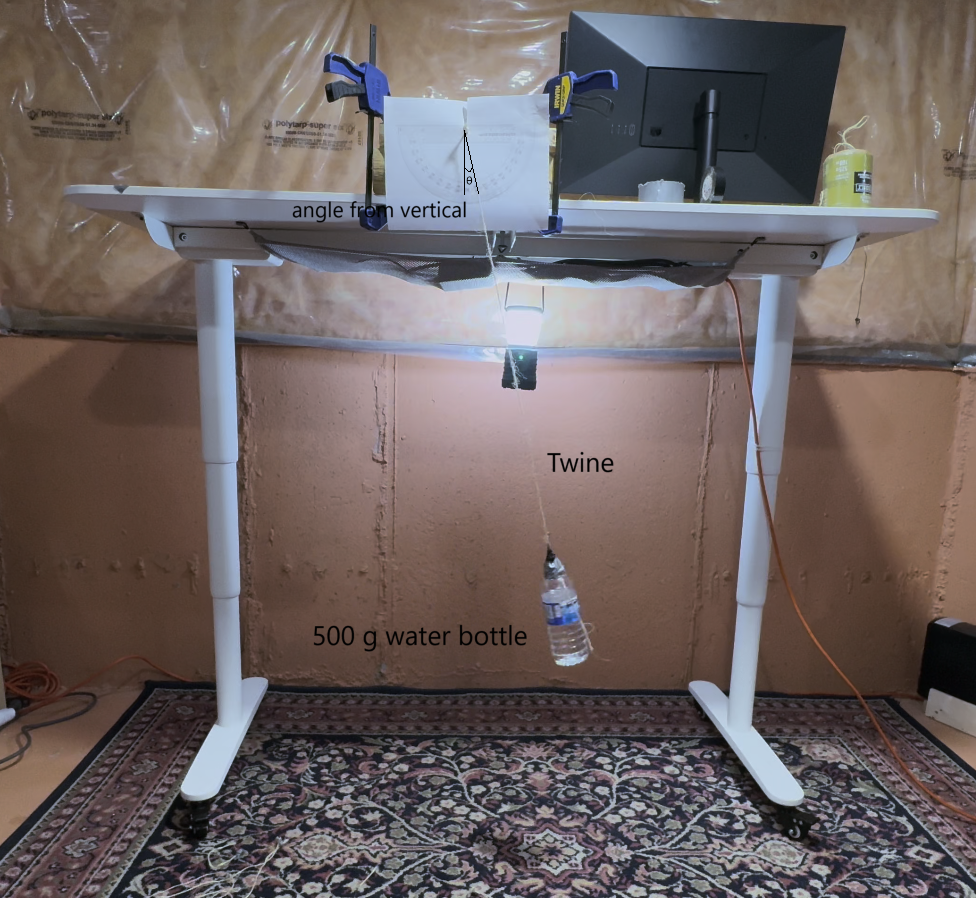
\includegraphics[width=\linewidth]{temp.png}
        \caption{The experimental setup}
        \label{fig:setup}
    \end{figure}
    \textcolor{Plum}{For part (i)}, an 85.0 $\pm$ \textcolor{WildStrawberry}{0.5} cm jute twine string with mass $<$ 10.0 $\pm$ 0.1 g was tied from one end to a 500 mL plastic water bottle filled with water to a mass of \textcolor{WildStrawberry}{500.0} $\pm$ 0.1 g. The other end of the jute twine was tied to a nail 100.0 $\pm$ \textcolor{WildStrawberry}{0.5 cm} above the ground. The jute twine was tied tightly so there was no visible slipping when the mass swung. To record the motion of the pendulum, a smartphone camera was positioned 120.0 $\pm$ \textcolor{WildStrawberry}{0.5 cm} away from the pendulum setup. The camera recorded video at 30 FPS and its video was inputted into an application called \textit{Tracker} which automatically tracked the horizontal and vertical position of the pendulum with time. To calibrate the distance scale in the tracker application, a piece of 28.0 $\pm$ 0.5 cm paper was placed on the plane of the pendulum motion. The origin of the coordinate system was the center of the video frame. Black tape was placed on the water bottle to help the AutoTracker distinguish the water bottle from the light-coloured background. 
    Data from \textit{Tracker} was processed and graphed using a script provided by Wilson with some modifications (see Appendix).
    The mass was swung from 1.40 $\pm$ 0.01 rad to -1.40 $\pm$ 0.01 rad in increments of 0.35 $\pm$ 0.01 rad. The Tracker application plots a position-time graph, and the period was measured from this graph by taking the time it takes for 10 oscillations to complete and dividing by 10. This data is included in the Appendix and was processed to determine the relationship between release angle (part (i)). The same data was used to determine the Q factor of the pendulum (part (ii)).
    \textcolor{Plum}{The experimental setup for part (iii) is the same except the mass is swung from 0.52 $\pm$ 0.01 rad every trial, and the length of the string is varied from 20.0 $\pm$ 0.5 cm to 85.0 $\pm$ 0.5 cm. All uncertainties in graphs were propagated by the code Wilson provided (see Appendix)} % increments.... not consistent 


    \section*{Part (i) Testing for Symmetry}
    Wilson's model suggests that the period of the pendulum is independent to the pendulum's release angle (Equation 1). The data is summarized in \cref{fig:symmetryTest}.

    \begin{figure}[H]
        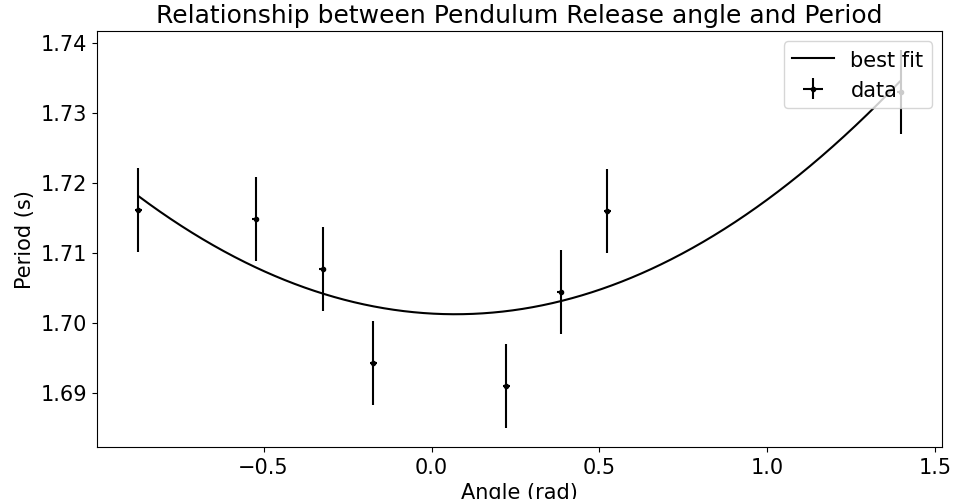
\includegraphics[width=\linewidth]{pendulum_release_angle_vs_period.png}
        \caption{The period of the pendulum depend on the release angle from the vertical. The line of best fit as calculated by the provided Python code \cite{Wilson} was (0.02 $\pm$ 0.04)$\theta^2$ - (0.003 $\pm$ 0.005)$\theta$ + 1.70 $\pm$ 0.03. Horizontal error bars are not visible at this scale.}
        \label{fig:symmetryTest}
    \end{figure}

    \subsection*{\textcolor{WildStrawberry}{Analysis and Uncertainties}}
    \color{WildStrawberry}
    \cref{fig:symmetryTest} suggests that the pendulum depends on the release angle from the vertical. Importantly, since the curve fit has a second order term, $-\theta$ and $\theta$ have the same period indicating that the setup is symmetrical. Note that for the first and second order terms, the uncertainty is greater than its value. We deduce that these values are experimentally zero, which suggests that the period of a pendulum is effectively constant. This deduction is valid for data range tested, which is important to consider because larger release angles make the pendulum mass swing faster, meaning quadratic drag forces may affect the period independence from release angle.

    Both type A and type B uncertainties were considered. For period measurements, the type A uncertainty was calculated as the standard deviation in period across 5 trials of one data point. The type B uncertainty is the length of a quarter frame (as taught in class), which equals $1/120 \rm{s} = 0.008 \rm{s}$. I multiplied this uncertainty by 8 ($0.008 \times 8 = 0.06$, or the length of two frames). This accounts for human error because I had difficulty pinpointing when the pendulum period endpoint. 
    The Type A uncertainty in release angle was 0 since the pendulum mass was set to the same angle each trial. The type B uncertainty came from the protractor which measured in increments of $2^\circ$, which meant the uncertainty was $0.5^\circ = 0.009$ rad. 
    For both the period and angle measurements, the type B uncertainty was greater than the type A uncertainty, so that value was used. 

    \section*{Part (ii) Empirically determined Q factor}
    \textcolor{WildStrawberry}{In part (i) we found that the release angle of the pendulum is approximately independent to its period. So, any part (i) trial can be used to calculate $Q$ and I chose an angle 0.34 $\pm$ 0.01 rad because it was easy set up.}

    $Q$ is related to the exponential decay of amplitude with time so amplitudes of any position-time graph were plotted and an exponential best fit line was drawn (\cref{fig:amplitudeTgraph}). 

    \begin{figure}[H]
        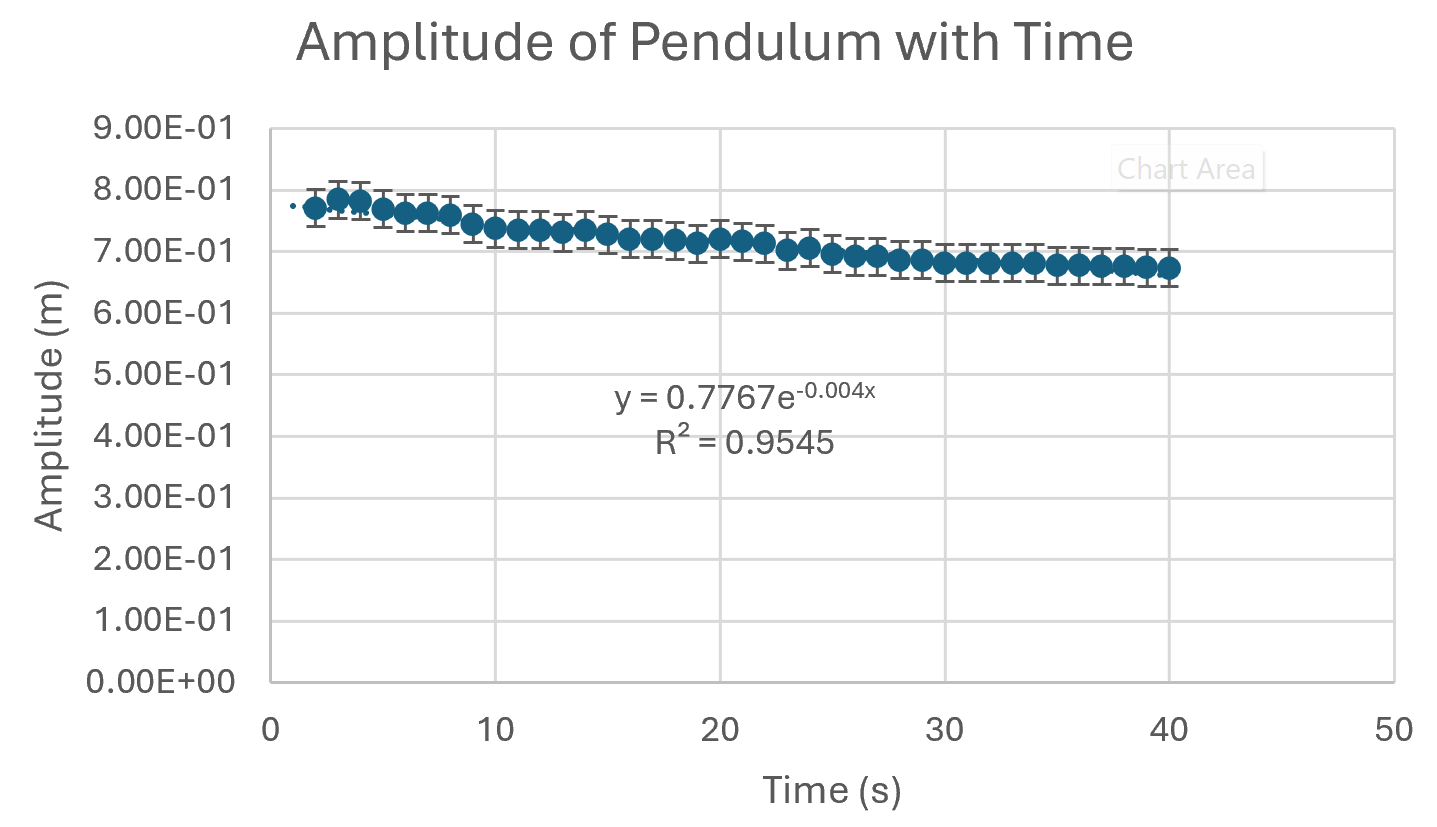
\includegraphics[width=\linewidth]{amplitudeTgraph.png}
        \caption{Graph of amplitude (m) vs time (s). Physlets Tracker was used to manually plot the location of the pendulum apexes with respect to time when the pendulum was at different angles from the vertical (-1.40, 1.40)$\pm$ 0.01 rad. The graph suggests that $\tau$ = 700 $\pm$ 100 \textcolor{WildStrawberry}{s}, and was calculated with the provided python script created by Wilson. Horizontal error bars are too small to be seen. The vertical error bars were calculated as half the width of the bottle cap}
        \label{fig:amplitudeTgraph}
    \end{figure}

    \subsection*{\textcolor{WildStrawberry}{Uncertainties and Analysis}}
    \color{Black}
    We used the experimental $\tau$ value to calculate the Q factor. Recall that $Q = \nicefrac{\tau \pi}{T} = \nicefrac{700\pi}{T} \pm (\nicefrac{100}{700})\times 100\% = 1300 \pm 200$. A Q factor of 270 $\pm$ 20 was also determined by counting the number of periods until the amplitude is $e^{-\pi}=4\%$ of its original amplitude. Since the Q factor is proportional to time, its percentage uncertainty matches the uncertainty in time.
    
    The two methods of calculating the Q factor give significantly different results, even while considering their uncertainties. I chose to use the counting method because the equation method assumes Wilson's theory is correct, but the counting method only assumes the pendulum motion is periodic. % unclear justification 

    For the uncertainties in amplitude of period, the type A uncertainty was the standard deviation across 5 trials, which was smaller than the type B uncertainty. It was calculated as half the width of the bottle cap = $24 mm / 2 = 12 mm \approx 0.01 m)$. This uncertainty is reasonable since Tracker tracked pixels on the bottle cap, so it could be at most 12 mm away from the pendulum center. 
    
    \section*{\textcolor{Plum}{Part (iii)a Relationship between Pendulum Length and Period}}
    \color{Plum}
    The pendulum mass was released from 0.52 $\pm$ 0.01 rad from the vertical at 5 different pendulum lengths and the data is summarized in \cref{fig:pendulumLengthVsPeriod}.
    \begin{figure}[H]
        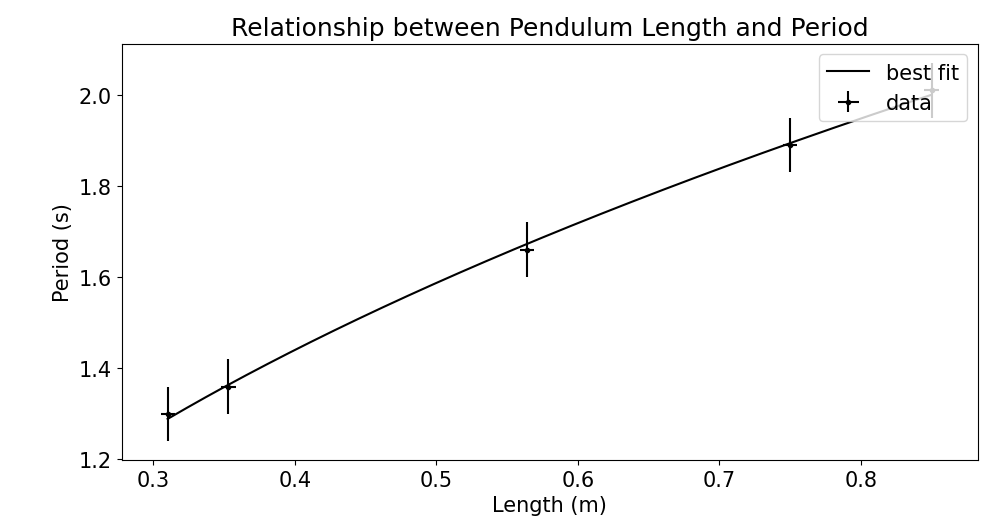
\includegraphics[width=\linewidth]{lengthvsperiodreal.png}
        \caption{\color{Plum} Graph of period vs. pendulum length (m) with a power law fit shows $T = (2.15 \pm 0.05)L^{0.44 \pm 0.06}$. Horizontal error bars are too small to be seen, and the vertical error bars is the uncertainty in period. }
        \label{fig:pendulumLengthVsPeriod}
    \end{figure} 
    The same data was also plotted on a log-log scale:
    \begin{figure}[H]
        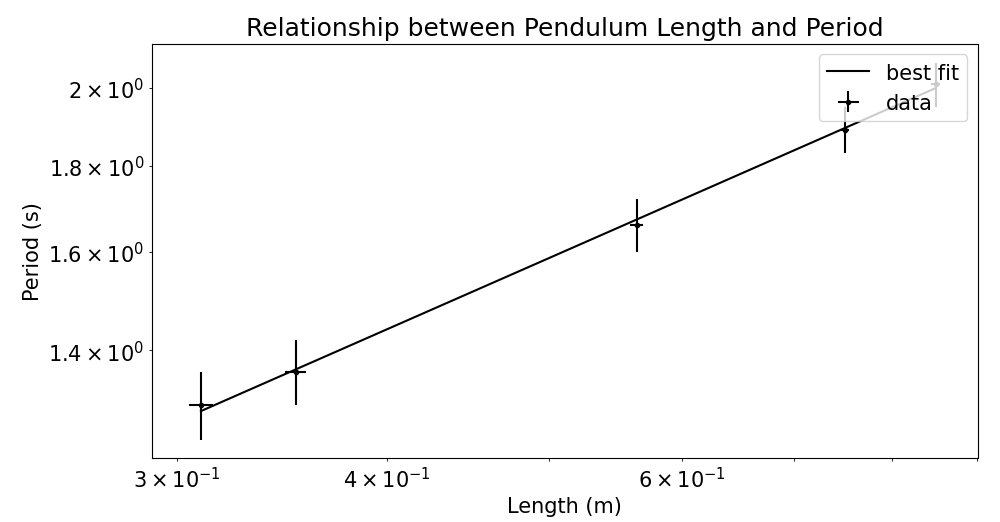
\includegraphics[width=\linewidth]{loglong-lengthvsperiodv2.png}
        \caption{\color{Plum} Graph of period vs. pendulum length (m) on a log-log scale. The log-log graph has a y-int of $2.15 \pm 0.05$ and slope of $0.44 \pm 0.06$. Horizontal error bars are too small to be seen, and the vertical error bars is the uncertainty in period. }
        \label{fig:loglog-pendulumLengthVsPeriod}
    \end{figure} 

    Compared to exponential, linear, and quadratic fits, the power law fit passed through the most error bars so was the most suitable curve fit function.

    \subsection*{Uncertainties and Analysis}
    Wilson predicted the power law best fit function to be $T = kL^n = 2L^{0.5}$. Our power law curve fit is $T = (2.15 \pm 0.05)^{0.44\pm 0.06}$. This disagrees with Wilson's prediction that $k = 2$ but agrees with $n=0.5$ within the uncertainties.  This data suggests that either Wilson's model is wrong by factor (perhaps damping force is a calculable constant), or there is a systematic error not accounted by uncertainties caused by the pendulum setup. 

    Type A uncertainties were once again tiny compared to type B uncertainties, because of a small standard of deviation between the results of 5 trials. Type B uncertainties in period are calculated in the same manner described in part (ii). The type B uncertainty in length was half the smallest increment of the measuring tool (measuring tape) = $\nicefrac{1}{2}\times 1$ cm. I used half instead of a quarter we learned in class because my camera was not perfectly in line with the pendulum setup. This uncertainty can be reduced by accounting for parallax error, so it is reasonable to use a smaller uncertainty. 
    
    \section*{\textcolor{Plum}{Part (iii)b Relationship between Pendulum Length and Q Factor}}
    \color{Plum}
    The data obtained in part (iii)a was used to calculate $Q$ for pendulum length using the counting method. The counting method, described in part (ii) was used because it is more reasonable for the data used.  $Q$ factor was graphed against pendulum length and a linear, quadratic, and exponential fit were applied. The linear fit was the appropriate fit since it passed through the most error bars. 
    \begin{figure}[H]
        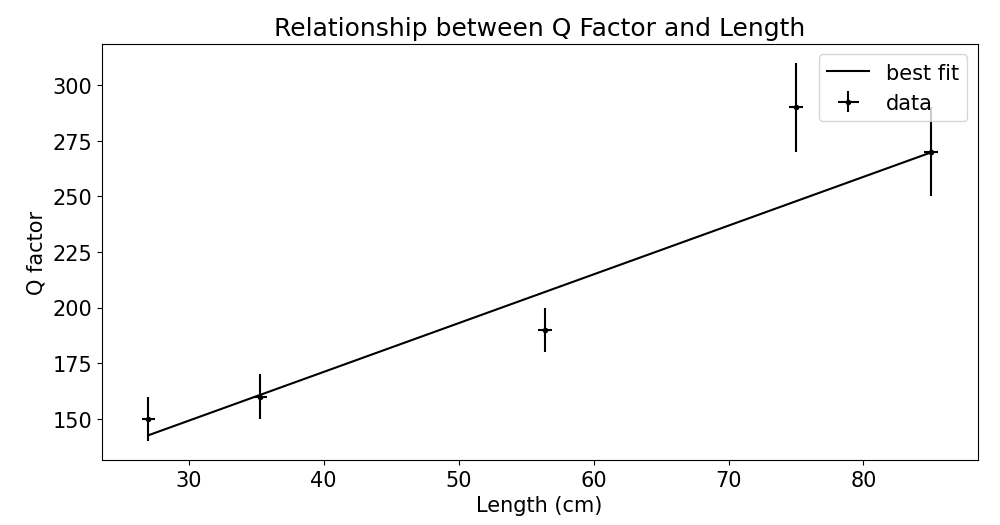
\includegraphics[width=\linewidth]{qfactorvslength.png}
        \caption{\color{Plum} Graph of Q factor vs. pendulum length (cm) with a linear fit shows that the Q factor scales linearly with the length of the pendulum. Horizontal error bars is the uncertainty in length and the vertical error bars is the uncertainty in $Q$ factor. The best fit line is $Q = (2.2 \pm 0.3)L + 80 \pm 10$, where $L$ is the length of the pendulum.  }
        \label{fig:qfactorvslength}
    \end{figure} 

    \subsection*{Uncertainties and Analysis}
    The $Q$ factor increases with pendulum length by the relation $Q = (2.2 \pm 0.3)L + 80 \pm 10$. However, the point at  75.0 $\pm$ 0.5 cm does not follow the linearly increasing trend. This data point could be a measurement error, but that is unlikely since multiple trials were taken. We conclude a greater range of lengths needs to be measured to develop a conclusive relation between $Q$ factor and pendulum length.  

    The type A and type B uncertainties are the same for part (iii)a. Since $Q$ factor is proportional to time, the percentage uncertainties for time were used as percentage uncertainties of $Q$. Next time to reduce uncertainty, a higher frame rate camera could be used since it was noted in part (ii) that the uncertainty in time came from difficulty pinpointing the end of the period. A higher frame rate camera would make the motion smoother and easier to pinpoint. 

    \color{Black}

    \subsection*{Discussion}
    \textcolor{Plum}{\textcolor{Red}{\textbf{Edits were made to improve flow in this section}} The experimental results from parts (i), (ii), (iii)a and suggest that Wilson's model is partially correct. The difference between theory and result may be from methodology errors.} For instance, I assumed parallax error would not affect trends in data but may have introduced an error factor. This may explain why in part (iii)a, the data disagreed with Wilson's model. There were also issues with Tracker's AutoTracker skipping frames and beginning to track the incorrect pixels. I accounted for this by increasing the uncertainty in amplitude, and manually tracked those frames in Tracker. Still, it suggests the current setup is suboptimal for software based tracking. Next time, the parallax error can be accounted for by calculations and reflective tape can be placed on the bottle so pixel tracking is consistent. 

    It may also be that Wilson's model is incorrect. Considering that the counting method was significantly smaller than the equation method suggests that Wilson's model did not consider all damping forces. Namely, friction between the string and nail, and drag forces. This model should always overpredict $Q$, which agrees with our data that $Q$ by counting is less than $Q$ by the equation. Next time, numerical modelling can be used to predict quadratic drag on the mass.

    Lastly, the pendulum started to oscillate off-axis despite attempts to minimize it by lining up the mass in the plane of the pivot point. This meant part of the pendulum decay was a result of energy being converted to rotation, which would increase the decay rate, or reduce $Q$. Next time, a light rod coupled with a heavier mass could be used with a hinge so the pendulum oscillates desirably.
    \section*{Conclusion}
    \color{WildStrawberry}
    This experiment was split into three parts to test the validity of Wilson's model that predicts the behaviour of a pendulum. We constructed a pendulum with household materials to gather data from.
    
    In part (i) we found Wilson's prediction that period is independent of release angle to be valid for the range of angles tested. 
    In part (ii), we determined the $Q$ factor for our pendulum was $270 \pm 20$ by the counting method or $1300 \pm 200$ which assumes Wilson's model is correct. The counting method was deemed more accurate since it does not rely on the validity of Wilson's model which suggests it's not perfect.
    In part (iii)a, an experiment found the relation between period and pendulum length to be $T = (2.15 \pm 0.05)^{0.44\pm 0.06}$ which differs from Wilson's model.
    In part (iii)b, $Q$ factor was plotted against pendulum length to get $Q = (2.2 \pm 0.3)L + 80 \pm 10$ from the most suitable curve fit function. One $Q$ data point decreased with length instead of increasing which suggests a greater data range is needed to make a conclusion about the $Q$ factor-length trend.
    
    The data suggests Wilson's model is partially correct; a better model would account for quadratic damping forces.
    \color{Black}

    \begin{thebibliography}{}

    \bibitem{OpenStax}
    OpenStax. (n.d.). \textit{15.5 Damped Oscillations | University Physics Volume 1}. Retrieved from \url{https://courses.lumenlearning.com/suny-osuuniversityphysics/chapter/15-5-damped-oscillations/}

    \bibitem{Wilson}
    Wilson. (2022). \textit{PHY180 Lab Project (2024)}. Retrieved from \url{https://q.utoronto.ca/courses/363836/files/32826310?module_item_id=6082503}

    \end{thebibliography}

    \section*{Appendix}
    All data and code is stored \href{https://github.com/PRU1/PHY180-pendulum-project}{here}.

\end{document}